\section{Introduction}
\renewcommand{\arraystretch}{1.5}
\begin{center}
    \begin{tabular}{l|l}
        CI/CD & Deployment environment, provides name and url for monitoring \\
        \hline
        Ansible & Installation and configuration of applications \\
        \hline
        Terraform & Provisioning of infrastructure \\
        \hline
        Kubernetes & Configuration + application: Deployment, scaling, managing workloads \\
        \hline
        Helm & Package- and Lifecycle Manager for K8s \\
        \hline
        Kustomize & Overlaying declarative specifications on top of existing K8s Manifests \\
        \hline
        Prometheus & Monitoring K8s Infrastructure and applications for reliability \\
        \hline
        Service Mesh & Traffic Management, Security, Observability and Service Discovery \\
        \hline
        GitOps & Everything as code, declarative system operation definition, control loop \\
    \end{tabular}
\end{center}

\subsection{DevOps}
\begin{figure}[h]
    \centering
    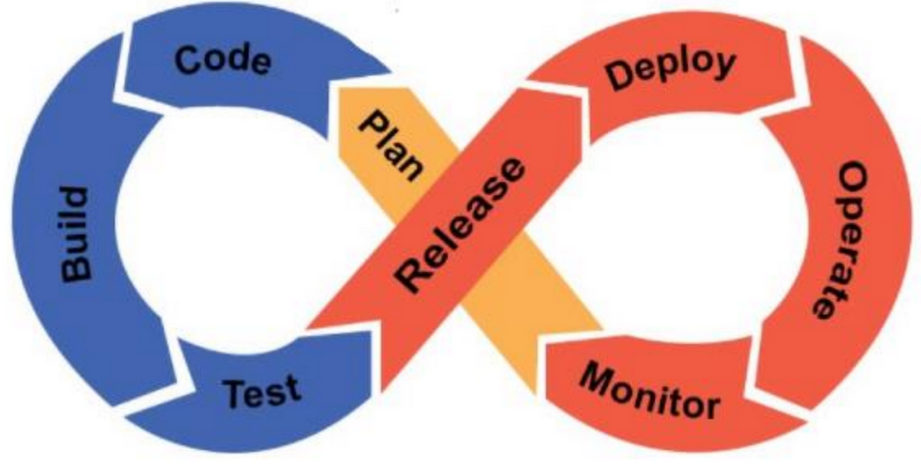
\includegraphics[width=8cm]{introduction-devops}
    \caption{DevOps Cycle}
\end{figure}

The DevOps pipeline focuses on Continuous Integration / Continuous Deployment. It applies a systems thinking and avoids
too much focus on only one piece of the workflow.

It values feedback, automated and personal to keep production healthy. Monitoring is an important type of automated feedback. 

Learning and continued experimentation lead to constantly improved systems and workflows.

\subsubsection{Plan}
Add objectives and requirements to the \textbf{backlog}, feedback from end users and operations team. 
Add backlog \textbf{tasks to sprints}. Track and plan activities using \textbf{board and project management tools}. 
\subsubsection{Code}
Code from all developers gets integrated into a \textbf{central source code repository}. 
\subsubsection{Build}
\textbf{Continuous Integration pipeline} is invoked every time code is pushed into the central repository. 
Includes \textbf{automated unit and integration tests}. Only after successful build and test, code can be reviewed and merged.     
\subsubsection{Test}
Automated deployment of code into a testing environment. Tests executed include \textbf{load, accessibility, performace and end-to-end testing}. 
Manual work like \textbf{user acceptance testing} also usually happens at this stage.    

\subsubsection{Release}
Tag a snapshot of the code with a \textbf{semantic versioning number}. Changes, features, breaking changes and deprecated features are documented.
Release can include artifacts such as \textbf{binaries} and \textbf{packages}. 

\subsubsection{Deploy}
Installs release into \textbf{production environment}. Can be automated or manual.

\subsubsection{Operate}
Infrastructure and Operations team ensure \textbf{smooth operation of the product}. \textbf{Scaling infrastructure} to meet demands.

Issues in infrastructure can be troubleshooted and resolved. \textbf{Document issues} for next planning stages. 

\subsubsection{Monitor}
\textbf{Collect data} on usage, performance, errors and more. Data collected is used for next iteration of DevOps cycle.

\subsection{Automated DevOps with GitLab CI}

Using GitLab CI pipeline, code can be built, tested and deployed automatically on every change. 
Tasks are defined in .gitlab-ci.yml file kept together with the code repository. 

\subsubsection{Integrating Kubernetes}

\subsubsection{Auto-DevOps: Setup with zero configuration}

\subsubsection{Creating gitlab CI Configuration}

\subsubsection{Testing with Docker}